%!TeX program = xelatex
\documentclass{SYSUReport}
\usepackage{listings}
\usepackage{hyperref}


\headl{多功能计算器}
\lessonTitle{面向对象程序设计课程设计}
\reportTitle{多功能计算器}
\stuname{白昊臻 \quad 杨宇鹤}
\stuid{231870175 \quad 231870155}
\inst{工程管理学院 \quad 软件学院}
\major{工业工程 \quad 软件工程}
\date{\today}




\begin{document}

% =============================================
% Part 1: 封面
% =============================================
\cover
\thispagestyle{empty} % 首页不显示页码
\clearpage

% =============================================
% Part 3: 目录页
% =============================================
% 重置页码,并使用罗马数字
\pagenumbering{Roman}
\setcounter{page}{1}
\tableofcontents
\clearpage
% =============================================
% Part 4: 正文内容
% =============================================
% 重置页码,并使用阿拉伯数字
\pagenumbering{arabic}
\setcounter{page}{1}


\section{系统需求分析}

\subsection{项目目标}
本项目的目标是从零实现一个科学计算器,支持实数与分数的四则运算以及常见函数运算,并提供可视化交互界面。
计算器的详细功能如下:

\begin{enumerate}
    \item 实数与实数、实数与分数、分数与分数的加、减、乘、除运算。
    \item 通过括号控制运算优先级。
    \item 常用函数,包括阶乘、幂函数、开方、倒数、三角函数、对数函数。
    \item 提供常用的矩阵运算操作,包括矩阵的加法、减法、乘法。
    \item 提供数据库连接,并对数据进行描述性统计,保存统计数据。
\end{enumerate}

总之,本计算器最终的目标是实现覆盖当前手机自带计算器的所有功能,并另外集成矩阵与数据库的操作,并且方便使用。

\subsection{功能说明}

\begin{figure}[!htbp]
    \centering
    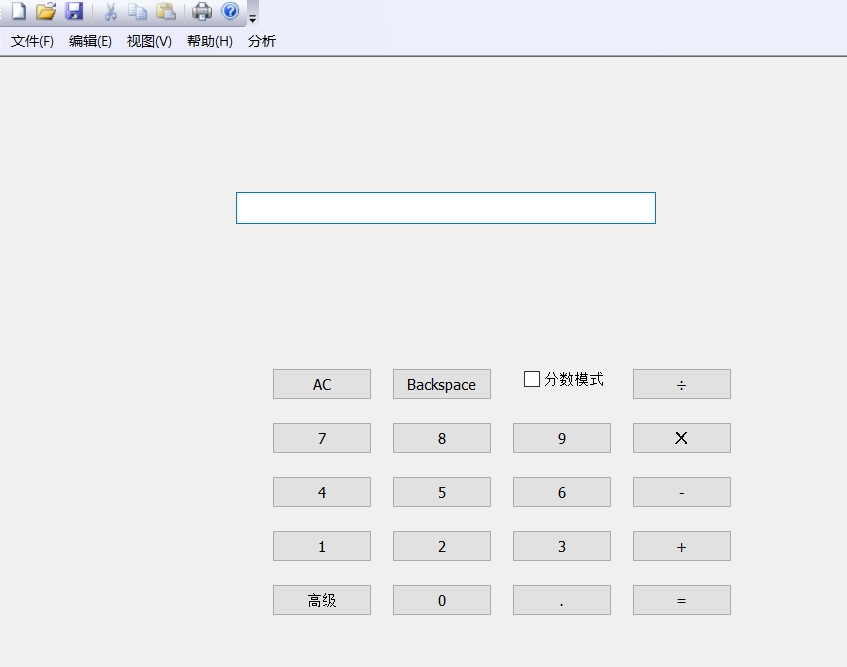
\includegraphics[width = 12cm]{MainPage.jpg}
    \caption{主界面}
    \label{fig:Dialog}
\end{figure}
计算器的基本界面如\autoref{fig:Dialog}所示,设计仿照现代手机自带的计算器,基础使用方法完全相同,
用户通过点击对应按钮向编辑框中输入算式,点击“=”,可以计算并把结果显示在编辑框。
勾选“分数模式”,可以输入分数,并且运算结果也都用分数表示
(此处的分数四则运算不是浮点数的近似表示,而是完全精确的)。

\begin{figure}[!htbp]
    \centering
    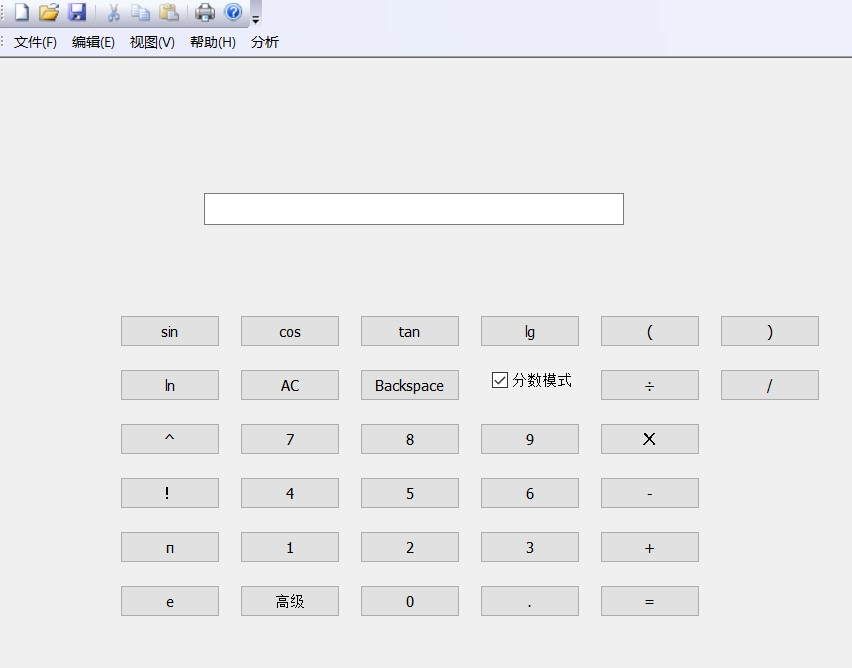
\includegraphics[width = 12cm]{高级.jpg}
    \caption{高级主界面}
    \label{fig:Advance}
\end{figure}
如果点击“高级”,则会显示常用的科学计算符号,如\autoref{fig:Advance}所示。

\begin{figure}[!htbp]
    \centering
    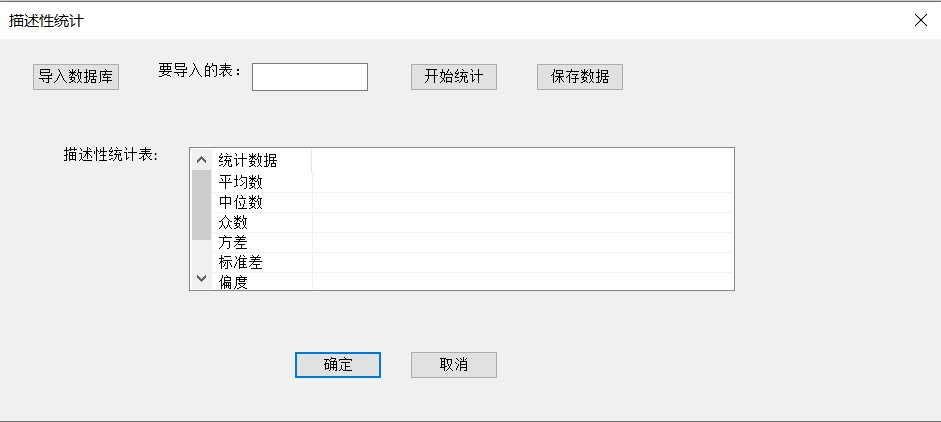
\includegraphics[width = 12cm]{描述性统计.jpg}
    \caption{描述性统计界面}
    \label{fig:DesStat}
\end{figure}
\begin{figure}[!htbp]
    \centering
    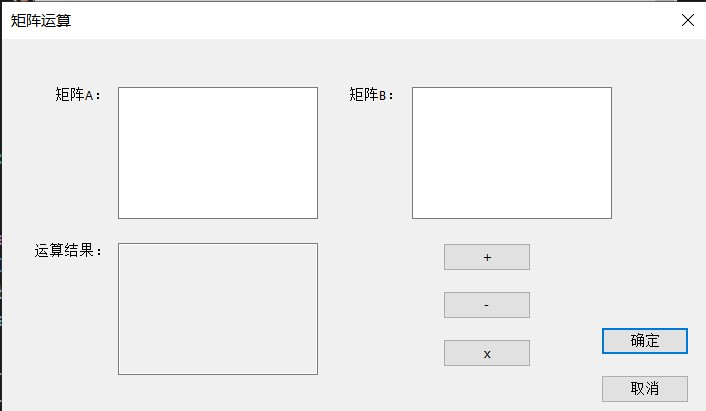
\includegraphics[width = 12cm]{矩阵运算.jpg}
    \caption{矩阵运算界面}
    \label{fig:MatrixManip}
\end{figure}
在菜单栏,提供了“高级”选项,可以选择“描述性统计”或“矩阵运算”,点击后会弹出相应对话框,如\autoref{fig:DesStat} 和 
\autoref{fig:MatrixManip}所示。
   
在“描述性统计”中,点击导入数据库,会打开文件浏览窗口;选择数据库文件后,填写
要统计的表,点击“开始统计”,
程序以每列作为一个指标,计算各列的描述统计数据,包括平均数、中位数、众数、
方差、标准差、偏度、峰度(自动忽略第一列ID),点击“保存数据”,可以保存至txt文件。

在“矩阵运算”中,以空格分隔行向量中不同数据,以换行分隔不同行向量;点击相应按钮得到计算结果。
    
\section{总体设计}

多功能计算器的主页面功能设计如\autoref{fig:Overall}所示。
\begin{figure}[!htbp]
    \centering
    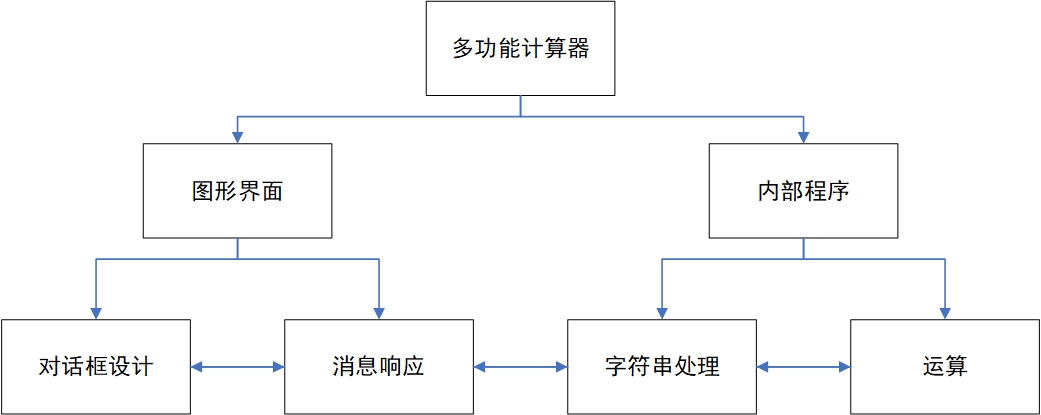
\includegraphics[width = 15cm]{总体设计图.jpg}
    \caption{总体设计图}
    \label{fig:Overall}
\end{figure}

其中,对话框、消息响应函数、字符串处理程序与运算程序均包含双向信息传递。在
单次运算中,用户通过图形界面输入算式,点击“=”后,算式字符串从编辑框被读取,
传递至字符串处理函数转化为数字与符号序列,再由运算程序计算结果;计算的结果返回
消息响应函数,实现对话框更新。

值得一提的是,本项目在菜单中增加了“描述性统计”和“矩阵运算”选项,这两个功能相对独立,
但仍然大致采用上图的信息处理流程。

\subsection{对话框}
如1.2节\autoref{fig:Advance},\autoref{fig:DesStat},\autoref{fig:MatrixManip}所示。


\subsection{消息处理函数}

对话框每一个控件都有单独的消息处理函数,根据功能可以分为三类,分别是:
\begin{enumerate}
    \item “=”的消息处理函数,负责获取编辑框算式,传递给字符串处理函数,并更新结果至编辑框;
    \item “高级”和“分数模式”的消息处理函数,负责管理对话框中按钮的显示与否,以及运算模式;
    \item 其余按钮的消息处理函数,负责输入算式。
\end{enumerate}

另外,还有菜单中选项的消息处理程序,其功能是创建对应的对话框。

\subsection{字符串处理程序与运算程序}
主界面的字符串处理与运算在逻辑上是两个分步过程,但实际中,我们利用栈实现了字符串解析与运算的并行化,
从而能很好地处理运算优先级。

“描述性统计”或“矩阵运算”的字符串处理和运算是分开进行的,比主界面更简单。

\subsection{难点}
本项目难点在于字符串解析和运算,因为有优先级和括号的存在,计算没有固定的顺序,所以必须实时解析并运算。

\lstset{
  breaklines=true,
  basicstyle=\footnotesize\ttfamily,
  language=C++,                % 设置语言
  basicstyle=\ttfamily,        % 设置代码字体
  keywordstyle=\color{blue},   % 设置关键字颜色
  stringstyle=\color{red},     % 设置字符串颜色
  commentstyle=\color{green},  % 设置注释颜色
  morecomment=[l][\color{magenta}]{\#}  % 预处理器指令颜色
}
\section{详细设计}
本节将结合具体代码,详细阐述每个环节的设计思路,具体实现方式。

\subsection{整体框架}
本项目使用了VS2022的MFC单文档框架,选择了View类,并继承CFormView类。这样可以在生成菜单的同时,在主界面添加控件。
项目使用到的类如\autoref{fig:AllClasses}所示,
\begin{figure}[!htbp]
    \centering
    \includegraphics[width = 15cm]{类.jpg}
    \caption{总体设计图}
    \label{fig:AllClasses}
\end{figure}

\begin{itemize}
    \item CalculatorView类负责接受所有主界面控件的消息并执行相应操作。
    \item DoWithString是.cpp文件,提供了CalculatorView类中声明的
    applyOp、precedence、evaluate等函数的实现,这些函数共同实现了
    解析并计算传入的算式字符串,返回结果。
    \item Fraction类实现分数数据类型。
    \item CDescribeStat和CMatrixManip分别是菜单功能“描述性统计”和“矩阵运算”对话框
        的关联类,负责实现对话框中控件的消息响应和功能
\end{itemize}

\subsection{CalculatorView类}
本小节依照用户信息的输入顺序阐述消息传递的具体实现。在设计之初,为CalculatorView添加
CString成员变量m\_input用于储存用户在编辑框输入的字符串。
现在假设用户要计算$1+2$,
当用户点击按钮"1",系统会调用CalculatorView中其对应的消息响应函数:
\begin{lstlisting}
    void CCalculatorView::OnBnClickedButton1()
    {
        m_input += _T("1");
        UpdateData(FALSE);
    }
\end{lstlisting}
此函数将字符“1”添加在m\_input末尾,并将m\_input的值在窗口更新。"+"和"2",以及其他所有
数字和运算符的函数都同理。

在这之后,用户会点击“=”,对应的消息响应函数如下:
\begin{lstlisting}
    void CCalculatorView::OnBnClickedButtonEqual()
    {
	if (m_FractionMode.GetCheck() == BST_UNCHECKED) {
		evaluate(m_input, 1);
	}
	else {
		evaluate(m_input, 2);
	}
	UpdateData(FALSE);
    }
\end{lstlisting}
m\_FractionMode也是CalculatorView类的成员变量,其关联对话框中的“分数模式”
勾选状态,通过检测其状态来确定evaluate函数的模式,evaluate负责计算结果并更新m\_input。
至此,完成了$1+2$的计算。

在点击菜单中“表述性统计”时,调用下面的函数:
\begin{lstlisting}
    void CCalculatorView::OnStatDescribe()
    {
	    CDescribeStat ds;
	    ds.DoModal();
    }
\end{lstlisting}
此函数调用CDescribeStat类的DoModal函数,生成新的对话框,“矩阵运算”
同理。

为了实现“高级”中设置控件可见性的功能,引用了辅助函数
checkVisibility:
\begin{lstlisting}
    void CCalculatorView::checkVisibility(int ID)
    {
        // 检查控件当前是否可见
        CWnd* pControl = GetDlgItem(ID);
        if (pControl && pControl->IsWindowVisible())
        {
            pControl->ShowWindow(SW_HIDE);  // 当前可见则隐藏
        }
        else
        {
            pControl->ShowWindow(SW_SHOW);  // 当前隐藏则显示
        }
    }
\end{lstlisting}
利用此函数,可以轻易实现“高级”和“分数模式”的消息处理函数。

\subsection{Fraction类}
Fraction类负责提供分数数据类型,
支持分数的存储,四则运算,以及基本函数运算。
\begin{lstlisting}
    class Fraction
    {
    private:
        long long m_numerator;
        long long m_denominator;
    public:
        //构造函数
        explicit Fraction(long long above = 0, long long below = 1); 
        Fraction(const Fraction& rhs); //复制构造函数
        Fraction(long double input); //小数转化成分数
        void reset(long long above, long long below); //重置分数值
        void gcd(); //化简
        long long up(); //返回分子的值
        long long down(); //返回分母的值
        friend Fraction operator+(const Fraction& left, 
            const Fraction& right);
        ...... // 四则运算符重载
        friend Fraction pow(Fraction& left, 
            Fraction& right);
        .... // 幂函数、对数函数等函数的重载
    };    
\end{lstlisting}
为了尽可能提高运算精度,分子和分母均为long long类型。大多数成员函数的
实现都比较简单,具体可查看附录,此处具体解释小数转分数的构造函数实现:
\begin{lstlisting}
    Fraction::Fraction(long double decimal) {
        // 取传入小数的整数部分
        long long intPart = static_cast<long long>(decimal);
        if (intPart == decimal) {
            // 整数部分等于整体,说明小数部分为0,传入的是整数
            m_denominator = 1;
            m_numerator = intPart;
        }
        else {
            const long precision = 1000000; // 定义精度
            // 将传入小数乘以精度后取整,即得到分子
            this->m_numerator = static_cast<long long>(round(decimal * precision));
            this->m_denominator = precision;
    
        }
        // 化简以精度为分母的分数
        this->gcd();
    }
\end{lstlisting}
为了使转化后的分数视觉上直观,设置了转化精度。




\input{Chapter2/part5.tex}

\input{Chapter2/part6.tex}


\section{困难及解决方案}
本节将介绍开发过程中遇到的困难,以及解决方法。

\subsection{框架设计}
在开发之初,由于对MFC不够熟悉,我们遇到了许多奇怪的错误。
我们想找一个既有主菜单,又以对话框为主界面的框架,找寻好久
才找到基于单文档的继承CFormView类的MFC框架;
不知道要把预编译头文件"pch.h"放在头文件首位,
导致自己定义的类总是构建失败;因为不熟悉各个类具体的功能,
不知道应该在哪里添加消息处理函数。这些问题最终都通过查阅资料解决。

\subsection{消息处理}

\subsubsection*{特殊字符输入}

在编辑对话框的时候,首先遇到的问题就是如何输入并读取
除号、派等特殊字符,对此,我们查询了这些字符的Unicode
编码,直接使用编码来显示字符,如除号在代码中就是L'\textbackslash u00F7'。

\subsubsection*{纠错机制}

在测试过程中,会出现不小心连续输入两个运算符的情况,
比如“1++2”,这样计算程序会直接崩溃,为了增加程序健壮性,
我们增加了纠错机制,每次输入字符,程序都会检查是否出现连续的
运算符,如果出现,则忽略输入或为其添加括号,具体程序如下:
\begin{lstlisting}
    void CCalculatorView::OnEnChangeEdit()
    {
        int length = m_input.GetLength();
        wchar_t last = m_input[length - 1], 
            second = m_input[length - 2];
        // 如果倒数第二个符号不是“-”
        if (second == L'+' || second == L'\u00D7' || second == L'\u00F7') {
            // 置换为倒数第一个字符
            if (last == L'+' || last == L'\u00D7' || last == L'\u00F7') {
                m_input.Delete(length - 2);
            } 
            // 如果倒数第一个字符是“-”,当成符号,为其加括号
            else if (last == L'-') {
                m_input.Insert(length - 1, L'(');
            }	
        }
        // 如果倒数第二个符号是“-”,则置换为倒数第一个字符
        else if (second == L'-') {
            if (last == L'-' || last == L'+' || last == L'\u00D7' || last == L'\u00F7') {
                m_input.Delete(length - 2);
            }
        }
        UpdateData(FALSE);
    }
\end{lstlisting}

\subsection{字符串处理与运算}
起初,我们的分数类使用int类型作为分子和分母;使用double类型读取小数。
但实际测试中,我们发现运算很容易溢出(超过十亿就会溢出)。为了解决这个问题,
改用long long类型作为分子和分母;使用long double类型读取小数,实测改进后
支持$10^{18}$以内的运算,覆盖了绝大多数使用范围。

在数量级较大时,人眼不易确定具体的位数,所以每三位数使用逗号分割(分数模式不适用)。

在读取字符串的时候还发现了一个错误,原先对于字符串中数字是这样读取的:
\begin{lstlisting}
    BOOL ifDecimal = FALSE;
    while (i < expression.GetLength() && (isdigit(expression[i]) || expression[i] == L'.' || expression[i] == L',')  ) {
        ......
        val = (val * 10) + (expression[i] - '0');
        if (ifDecimal) val /= 10;
        i++;
    }
\end{lstlisting}
但这样实际上无法正确处理小数部分,经过调试,修正为:
\begin{lstlisting}
    BOOL ifDecimal = FALSE;
    long  decimalDigit = 1; //小数位数
    while (i < expression.GetLength() && (isdigit(expression[i]) || expression[i] == L'.' || expression[i] == L',')  ) {
        ......
        val = (val * 10) + (expression[i] - '0');
        if (ifDecimal) decimalDigit *= 10;
        i++;
    }
    val /= decimalDigit;
\end{lstlisting}

\subsection{描述性统计}
在使用ControlList的过程中,遇到了奇怪的现象,即使文本超出窗口,也不会出现水平滚动条。
查阅资料无果,经过大量测试后,发现只有初始状态有竖直滚动条,才能出现水平滚动条。
在进行数据保存时,我们遇到了编码问题,VS2022中MFC采用UTF-16进行编码,而Windows自带的
txt文本查看器采用UTF-8编码,直接保存会呈现乱码,查阅资料后我们加入了转码程序,使得数据正常保存。


\subsection{矩阵运算}
实现读取矩阵的程序时,我们忽略了windows中换行的独特表示,一开始我们用'\textbackslash n'表示换行符,
但没有作用,查阅资料后改为'\textbackslash r \textbackslash n',成功实现矩阵的读取。












\section{总结}
\subsection{不足}
\begin{itemize}
    \item 没有构建严格的输入纠错程序,如果输入的算式不符合数学格式,程序可能崩溃。
    \item 由于矩阵逆运算的复杂性,只提供了加、减、乘三种运算。
    \item 没能允许用户自主选择数据库中要统计的列,而是直接统计整个表格。
    \item 字符串处理程序没有很好地实现模块化,显得臃肿难以维护。
\end{itemize}

\subsection{收获}
\begin{itemize}
    \item 本次开发协作使用Git及Github完成,虽然过程中出现了登录失败等问题,
    但最终有效提高了效率,省去了使用队友代码时麻烦的配置工作,锻炼了合作开发的能力。
    \item 开发过程中查资料、调试,以及对代码整体框架的设计锻炼了工程能力。
    \item 增加了多文件程序以及窗口化程序的开发经验。
\end{itemize}
这次程序设计让我们意识到理论与实际之间地鸿沟,计算机、字符串处理地程序逻辑都不难理解,
可是要真正实现所有功能,解决各种奇奇怪怪的bug,提供可视化操作界面,需要数千行代码的支撑。
同时,这次作业也让我们熟练了C++类的用法,以及明白可视化程序的设计思路。理论指导实践,这次课程设计
是一次充实有趣的实践,让我们收益匪浅!








\section{附录}
本项目源代码已在Github开源,点击此\href{https://github.com/BHZ-boom/Calculator}{链接}查看。
因为MFC程序运行需要完整的框架,所以只复制源代码无法运行程序,建议直接在VS2022克隆GitHub仓库,
可以一键运行程序。
下面的附录只展示我们写的代码,没有MFC自动生成的代码文件。

CalculatorView.h
\begin{lstlisting}
// CalculatorView.h: CCalculatorView 类的接口
#pragma once

class CCalculatorView : public CFormView
{
protected: // 仅从序列化创建
    CCalculatorView() noexcept;
    DECLARE_DYNCREATE(CCalculatorView);

public:
#ifdef AFX_DESIGN_TIME
    enum{ IDD = IDD_CALCULATOR_FORM };
#endif

// 特性
public:
    CCalculatorDoc* GetDocument() const;

// 操作
public:

// 重写
public:
    virtual BOOL PreCreateWindow(CREATESTRUCT& cs);
protected:
    virtual void DoDataExchange(CDataExchange* pDX);    // DDX/DDV 支持
    virtual void OnInitialUpdate(); // 构造后第一次调用
    virtual BOOL OnPreparePrinting(CPrintInfo* pInfo);
    virtual void OnBeginPrinting(CDC* pDC, CPrintInfo* pInfo);
    virtual void OnEndPrinting(CDC* pDC, CPrintInfo* pInfo);
    virtual void OnPrint(CDC* pDC, CPrintInfo* pInfo);

// 实现
public:
    virtual ~CCalculatorView();
#ifdef _DEBUG
    virtual void AssertValid() const;
    virtual void Dump(CDumpContext& dc) const;
#endif

protected:

// 生成的消息映射函数与变量
protected:
    afx_msg void OnFilePrintPreview();
    afx_msg void OnRButtonUp(UINT nFlags, CPoint point);
    afx_msg void OnContextMenu(CWnd* pWnd, CPoint point);
    DECLARE_MESSAGE_MAP()
public:
    CString m_input;
    afx_msg void OnBnClickedButton0();
    afx_msg void OnBnClickedButton4();
    afx_msg void OnBnClickedButton6();
    afx_msg void OnBnClickedButton7();
    afx_msg void OnBnClickedButton1();
    afx_msg void OnBnClickedButton2();
    afx_msg void OnBnClickedButton3();
    afx_msg void OnBnClickedButton5();
    afx_msg void OnBnClickedButton8();
    afx_msg void OnBnClickedButton9();
    CButton markTimes;
    CButton markDivision;
    afx_msg void OnBnClickedButtonPlus();
    afx_msg void OnBnClickedButtonMinus();
    afx_msg void OnBnClickedButtonTimes();
    afx_msg void OnBnClickedButtonDivision();
    afx_msg void OnBnClickedButtonEqual();
    
public: //数据处理
    void evaluate(CString& expression, int mode);

private:
    template <typename T>
    T applyOp(T a, T b, wchar_t op);
    long double precedence(wchar_t op);
    void ConvertDouble(long double result, CString& input);
    
public:
    afx_msg void OnEnChangeEdit();
    afx_msg void OnBnClickedButtonPoint();
    afx_msg void OnBnClickedButtonBack();
    afx_msg void OnBnClickedButtonAc();
    CButton m_FractionMode;
    afx_msg void OnBnClickedButtonslash();
    afx_msg void OnBnClickedButtonAdvance();
    afx_msg void OnBnClickedCheckFraction();
    afx_msg void OnStatDescribe();
    afx_msg void OnBnClickedButtonFile();
    afx_msg void OnStatRegress();
    afx_msg void OnStatMatrix();
    afx_msg void OnBnClickedButtonRightp();
    afx_msg void OnBnClickedButtonLeftp();
    afx_msg void OnBnClickedButtonE();
    afx_msg void OnBnClickedButtonPi();
    afx_msg void OnBnClickedButtonF();
    afx_msg void OnBnClickedButtonPow();
    afx_msg void OnBnClickedButtonLn();
    afx_msg void OnBnClickedButtonLg();
    afx_msg void OnBnClickedButtonSin();
    afx_msg void OnBnClickedButtonCos();
    afx_msg void OnBnClickedButtonTan();
    void checkVisibility(int nID);
};

#ifndef _DEBUG  // CalculatorView.cpp 中的调试版本
inline CCalculatorDoc* CCalculatorView::GetDocument() const
    { return reinterpret_cast<CCalculatorDoc*>(m_pDocument); }
#endif    
\end{lstlisting}

CalculatorView.cpp
\begin{lstlisting}

// CalculatorView.cpp: CCalculatorView 类的实现
#include "pch.h"
#include "framework.h"
#include "CDescribeStat.h"
#include "CMatrixManip.h"
// SHARED_HANDLERS 可以在实现预览、缩略图和搜索筛选器句柄的
// ATL 项目中进行定义,并允许与该项目共享文档代码。
#ifndef SHARED_HANDLERS
#include "Calculator.h"
#endif

#include "CalculatorDoc.h"
#include "CalculatorView.h"

#ifdef _DEBUG
#define new DEBUG_NEW
#endif

// CCalculatorView

IMPLEMENT_DYNCREATE(CCalculatorView, CFormView)

BEGIN_MESSAGE_MAP(CCalculatorView, CFormView)
    // 标准打印命令
    ON_COMMAND(ID_FILE_PRINT, &CFormView::OnFilePrint)
    ON_COMMAND(ID_FILE_PRINT_DIRECT, &CFormView::OnFilePrint)
    ON_COMMAND(ID_FILE_PRINT_PREVIEW, &CCalculatorView::OnFilePrintPreview)
    ON_WM_CONTEXTMENU()
    ON_WM_RBUTTONUP()
    ON_BN_CLICKED(IDC_BUTTON_0, &CCalculatorView::OnBnClickedButton0)
    ON_BN_CLICKED(IDC_BUTTON_4, &CCalculatorView::OnBnClickedButton4)
    ON_BN_CLICKED(IDC_BUTTON_6, &CCalculatorView::OnBnClickedButton6)
    ON_BN_CLICKED(IDC_BUTTON_7, &CCalculatorView::OnBnClickedButton7)
    ON_BN_CLICKED(IDC_BUTTON_1, &CCalculatorView::OnBnClickedButton1)
    ON_BN_CLICKED(IDC_BUTTON_2, &CCalculatorView::OnBnClickedButton2)
    ON_BN_CLICKED(IDC_BUTTON_3, &CCalculatorView::OnBnClickedButton3)
    ON_BN_CLICKED(IDC_BUTTON_5, &CCalculatorView::OnBnClickedButton5)
    ON_BN_CLICKED(IDC_BUTTON_8, &CCalculatorView::OnBnClickedButton8)
    ON_BN_CLICKED(IDC_BUTTON_9, &CCalculatorView::OnBnClickedButton9)
    ON_BN_CLICKED(IDC_BUTTON_E, &CCalculatorView::OnBnClickedButtonE)
    ON_BN_CLICKED(IDC_BUTTON_Pi, &CCalculatorView::OnBnClickedButtonPi)
    ON_BN_CLICKED(IDC_BUTTON_PLUS, &CCalculatorView::OnBnClickedButtonPlus)
    ON_BN_CLICKED(IDC_BUTTON_MINUS, &CCalculatorView::OnBnClickedButtonMinus)
    ON_BN_CLICKED(IDC_BUTTON_TIMES, &CCalculatorView::OnBnClickedButtonTimes)
    ON_BN_CLICKED(IDC_BUTTON_DIVISION, &CCalculatorView::OnBnClickedButtonDivision)
    ON_BN_CLICKED(IDC_BUTTON_EQUAL, &CCalculatorView::OnBnClickedButtonEqual)
    ON_EN_CHANGE(IDC_EDIT, &CCalculatorView::OnEnChangeEdit)
    ON_BN_CLICKED(IDC_BUTTON_POINT, &CCalculatorView::OnBnClickedButtonPoint)
    ON_BN_CLICKED(IDC_BUTTON_BACK, &CCalculatorView::OnBnClickedButtonBack)
    ON_BN_CLICKED(IDC_BUTTON_AC, &CCalculatorView::OnBnClickedButtonAc)
    ON_BN_CLICKED(IDC_BUTTON_slash, &CCalculatorView::OnBnClickedButtonslash)
    ON_BN_CLICKED(IDC_BUTTON_ADVANCE, &CCalculatorView::OnBnClickedButtonAdvance)
    ON_BN_CLICKED(IDC_CHECK_FRACTION, &CCalculatorView::OnBnClickedCheckFraction)
    ON_COMMAND(ID_STAT_DESCRIBE, &CCalculatorView::OnStatDescribe)
    ON_COMMAND(ID_STAT_MATRIX, &CCalculatorView::OnStatMatrix)
    ON_BN_CLICKED(IDC_BUTTON_RIGHTP, &CCalculatorView::OnBnClickedButtonRightp)
    ON_BN_CLICKED(IDC_BUTTON_LEFTP, &CCalculatorView::OnBnClickedButtonLeftp)
    ON_BN_CLICKED(IDC_BUTTON_F, &CCalculatorView::OnBnClickedButtonF)
    ON_BN_CLICKED(IDC_BUTTON_Pow, &CCalculatorView::OnBnClickedButtonPow)
    ON_BN_CLICKED(IDC_BUTTON_Ln, &CCalculatorView::OnBnClickedButtonLn)
    ON_BN_CLICKED(IDC_BUTTON_Lg, &CCalculatorView::OnBnClickedButtonLg)
    ON_BN_CLICKED(IDC_BUTTON_Sin, &CCalculatorView::OnBnClickedButtonSin)
    ON_BN_CLICKED(IDC_BUTTON_Cos, &CCalculatorView::OnBnClickedButtonCos)
    ON_BN_CLICKED(IDC_BUTTON_Tan, &CCalculatorView::OnBnClickedButtonTan)
END_MESSAGE_MAP()

// CCalculatorView 构造/析构

CCalculatorView::CCalculatorView() noexcept
    : CFormView(IDD_CALCULATOR_FORM)
{
    m_input = _T("");
}

CCalculatorView::~CCalculatorView()
{
}

void CCalculatorView::DoDataExchange(CDataExchange* pDX)
{
    CFormView::DoDataExchange(pDX);
    DDX_Text(pDX, IDC_EDIT, m_input);
    DDX_Control(pDX, IDC_BUTTON_TIMES, markTimes);
    DDX_Control(pDX, IDC_BUTTON_DIVISION, markDivision);
    DDX_Control(pDX, IDC_CHECK_FRACTION, m_FractionMode);
}

BOOL CCalculatorView::PreCreateWindow(CREATESTRUCT& cs)
{
    // TODO: 在此处通过修改
    //  CREATESTRUCT cs 来修改窗口类或样式

    return CFormView::PreCreateWindow(cs);
}

void CCalculatorView::OnInitialUpdate()
{
    CFormView::OnInitialUpdate();
    GetParentFrame()->RecalcLayout();
    ResizeParentToFit();

    // 创建字体
    CFont font;
    font.CreatePointFont(100, _T("Segoe UI Symbol")); // 10号字体,使用 Segoe UI Symbol

    // 设置控件使用新字体
    CEdit* pEdit = (CEdit*)GetDlgItem(IDC_BUTTON_TIMES);
    pEdit->SetFont(&font);

    markTimes.SetWindowText(_T("\u00D7"));
    markDivision.SetWindowTextW(_T("\u00F7"));
    GetDlgItem(IDC_BUTTON_slash)->ShowWindow(SW_HIDE);
    GetDlgItem(IDC_BUTTON_Sin)->ShowWindow(SW_HIDE);
    GetDlgItem(IDC_BUTTON_Cos)->ShowWindow(SW_HIDE);
    GetDlgItem(IDC_BUTTON_Tan)->ShowWindow(SW_HIDE);
    GetDlgItem(IDC_BUTTON_Ln)->ShowWindow(SW_HIDE);
    GetDlgItem(IDC_BUTTON_Pow)->ShowWindow(SW_HIDE);
    GetDlgItem(IDC_BUTTON_F)->ShowWindow(SW_HIDE);
    GetDlgItem(IDC_BUTTON_Pi)->ShowWindow(SW_HIDE);
    GetDlgItem(IDC_BUTTON_E)->ShowWindow(SW_HIDE);
    GetDlgItem(IDC_BUTTON_LEFTP)->ShowWindow(SW_HIDE);
    GetDlgItem(IDC_BUTTON_RIGHTP)->ShowWindow(SW_HIDE);
    GetDlgItem(IDC_BUTTON_Lg)->ShowWindow(SW_HIDE);
}


// CCalculatorView 打印


void CCalculatorView::OnFilePrintPreview()
{
#ifndef SHARED_HANDLERS
    AFXPrintPreview(this);
#endif
}

BOOL CCalculatorView::OnPreparePrinting(CPrintInfo* pInfo)
{
    // 默认准备
    return DoPreparePrinting(pInfo);
}

void CCalculatorView::OnBeginPrinting(CDC* /*pDC*/, CPrintInfo* /*pInfo*/)
{
    // TODO: 添加额外的打印前进行的初始化过程
}

void CCalculatorView::OnEndPrinting(CDC* /*pDC*/, CPrintInfo* /*pInfo*/)
{
    // TODO: 添加打印后进行的清理过程
}

void CCalculatorView::OnPrint(CDC* pDC, CPrintInfo* /*pInfo*/)
{
    // TODO: 在此处添加自定义打印代码
}

void CCalculatorView::OnRButtonUp(UINT /* nFlags */, CPoint point)
{
    ClientToScreen(&point);
    OnContextMenu(this, point);
}

void CCalculatorView::OnContextMenu(CWnd* /* pWnd */, CPoint point)
{
#ifndef SHARED_HANDLERS
    theApp.GetContextMenuManager()->ShowPopupMenu(IDR_POPUP_EDIT, point.x, point.y, this, TRUE);
#endif
}


// CCalculatorView 诊断

#ifdef _DEBUG
void CCalculatorView::AssertValid() const
{
    CFormView::AssertValid();
}

void CCalculatorView::Dump(CDumpContext& dc) const
{
    CFormView::Dump(dc);
}

CCalculatorDoc* CCalculatorView::GetDocument() const // 非调试版本是内联的
{
    ASSERT(m_pDocument->IsKindOf(RUNTIME_CLASS(CCalculatorDoc)));
    return (CCalculatorDoc*)m_pDocument;
}
#endif //_DEBUG


// CCalculatorView 消息处理程序



void CCalculatorView::OnBnClickedButton0()
{
    m_input += _T("0");
    UpdateData(FALSE);
}

void CCalculatorView::OnBnClickedButton1()
{
    m_input += _T("1");
    UpdateData(FALSE);
}

void CCalculatorView::OnBnClickedButton2()
{
    m_input += _T("2");
    UpdateData(FALSE);
}

void CCalculatorView::OnBnClickedButton3()
{
    m_input += _T("3");
    UpdateData(FALSE);
}

void CCalculatorView::OnBnClickedButton4()
{
    m_input += _T("4");
    UpdateData(FALSE);
}

void CCalculatorView::OnBnClickedButton5()
{
    m_input += _T("5");
    UpdateData(FALSE);
}

void CCalculatorView::OnBnClickedButton6()
{
    m_input += _T("6");
    UpdateData(FALSE);
}


void CCalculatorView::OnBnClickedButton7()
{
    m_input += _T("7");
    UpdateData(FALSE);
}

void CCalculatorView::OnBnClickedButton8()
{
    m_input += _T("8");
    UpdateData(FALSE);
}

void CCalculatorView::OnBnClickedButton9()
{
    m_input += _T("9");
    UpdateData(FALSE);
}

void CCalculatorView::OnBnClickedButtonPoint()
{
    m_input += _T(".");
    UpdateData(FALSE);
}

void CCalculatorView::OnBnClickedButtonslash()
{
    m_input += _T("/");
    UpdateData(FALSE);
}



void CCalculatorView::OnBnClickedButtonPlus()
{
    m_input += _T("+");
    OnEnChangeEdit();
}


void CCalculatorView::OnBnClickedButtonMinus()
{
    m_input += _T("-");
    OnEnChangeEdit();
}


void CCalculatorView::OnBnClickedButtonTimes()
{
    m_input += _T("\u00D7");
    OnEnChangeEdit();
}


void CCalculatorView::OnBnClickedButtonDivision()
{
    m_input += _T("\u00F7");
    OnEnChangeEdit();
}


void CCalculatorView::OnBnClickedButtonEqual()
{
    if (m_FractionMode.GetCheck() == BST_UNCHECKED) {
        evaluate(m_input, 1);
    }
    else {
        evaluate(m_input, 2);
    }
    UpdateData(FALSE);
}


void CCalculatorView::OnEnChangeEdit()
{
    int length = m_input.GetLength();
    wchar_t last = m_input[length - 1], second = m_input[length - 2];
    if (second == L'+' || second == L'\u00D7' || second == L'\u00F7') {
        if (last == L'+' || last == L'\u00D7' || last == L'\u00F7') {
            m_input.Delete(length - 2);
        } 
        else if (last == L'-') {
            m_input.Insert(length - 1, L'(');
        }	
    }
    else if (second == L'-') {
        if (last == L'-' || last == L'+' || last == L'\u00D7' || last == L'\u00F7') {
            m_input.Delete(length - 2);
        }
    }
    UpdateData(FALSE);
}


void CCalculatorView::OnBnClickedButtonBack()
{
    if (!m_input.IsEmpty()) {
        m_input.Delete(m_input.GetLength() - 1);
    }
    UpdateData(FALSE);
}


void CCalculatorView::OnBnClickedButtonAc()
{
    m_input = _T("");
    UpdateData(FALSE);
}

void CCalculatorView::OnBnClickedButtonRightp()
{
    m_input += _T(")");
    UpdateData(FALSE);
}

void CCalculatorView::OnBnClickedButtonLeftp()
{
    m_input += _T("(");
    UpdateData(FALSE);
}

void CCalculatorView::checkVisibility(int ID)
{
    // 检查控件当前是否可见
    CWnd* pControl = GetDlgItem(ID);
    if (pControl && pControl->IsWindowVisible())
    {
        pControl->ShowWindow(SW_HIDE);  // 当前可见则隐藏
    }
    else
    {
        pControl->ShowWindow(SW_SHOW);  // 当前隐藏则显示
    }
}

void CCalculatorView::OnBnClickedButtonAdvance()
{
    checkVisibility(IDC_BUTTON_Sin);
    checkVisibility(IDC_BUTTON_Cos);
    checkVisibility(IDC_BUTTON_Tan);
    checkVisibility(IDC_BUTTON_Ln);
    checkVisibility(IDC_BUTTON_Pow);
    checkVisibility(IDC_BUTTON_F);
    checkVisibility(IDC_BUTTON_Pi);
    checkVisibility(IDC_BUTTON_E);
    checkVisibility(IDC_BUTTON_LEFTP);
    checkVisibility(IDC_BUTTON_RIGHTP);
    checkVisibility(IDC_BUTTON_Lg);
}


void CCalculatorView::OnBnClickedCheckFraction()
{
    checkVisibility(IDC_BUTTON_slash);
}


void CCalculatorView::OnStatDescribe()
{
    CDescribeStat ds;
    ds.DoModal();
        
}

void CCalculatorView::OnStatMatrix()
{
    CMatrixManip mm;
    if (mm.DoModal() == IDOK) {
        // 用户点击了OK,处理数据
    }
}

void CCalculatorView::OnBnClickedButtonE()
{
    m_input += _T("e");
    UpdateData(FALSE);
}


void CCalculatorView::OnBnClickedButtonPi()
{
    m_input += _T("π");
    UpdateData(FALSE);
}


void CCalculatorView::OnBnClickedButtonF()
{
    m_input += _T("!");
    UpdateData(FALSE);
}


void CCalculatorView::OnBnClickedButtonPow()
{
    m_input += _T("^");
    UpdateData(FALSE);
}


void CCalculatorView::OnBnClickedButtonLn()
{
    m_input += _T("ln");
    UpdateData(FALSE);
}


void CCalculatorView::OnBnClickedButtonLg()
{
    m_input += _T("lg");
    UpdateData(FALSE);
}


void CCalculatorView::OnBnClickedButtonSin()
{
    m_input += _T("sin");
    UpdateData(FALSE);
}


void CCalculatorView::OnBnClickedButtonCos()
{
    m_input += _T("cos");
    UpdateData(FALSE);
}


void CCalculatorView::OnBnClickedButtonTan()
{
    m_input += _T("tan");
    UpdateData(FALSE);
}    
\end{lstlisting}

DoWithString.cpp
\begin{lstlisting}
#include "pch.h"
#include <stack>
#include <cctype>
#include <string>
#include <cmath> 
#include <iostream>
#include <sstream>
#include <iomanip>
#include <locale>
#include <stdexcept>
#include <type_traits>
#include "framework.h"
#include "Calculator.h"
#include "CalculatorDoc.h"
#include "CalculatorView.h"
#define E     L"2.7182818"
#define Pi    L"3.1415926"

long double factorial(long double n) {
    if (n == 0) {
        return 1;
    }
    else {
        return n * factorial(n - 1);
    }
}

// Function to perform arithmetic operations.
template <typename T>
T CCalculatorView::applyOp(T a, T b, wchar_t op) {
    switch (op) {
        case L'+': return a + b;
        case L'-': return a - b;
        case L'*': return a * b;
        case L'/': return a / b;
        case L'^':return pow(a, b);
        case L'n':return log(a);
        case L'g':return log10(a);
        case L's':return sin(a);
        case L'c':return cos(a);
        case L't':return tan(a);
        default: throw std::invalid_argument("Invalid operator.");
    }
}

// Function to return precedence of operators
long double CCalculatorView::precedence(wchar_t op) {
    if (op == L'+' || op == L'-') return 1;
    if (op == L'*' || op == L'/') return 2;
    if (op == L'n' || op == L'g' || op == L's' || op == L'c' || op == L't') return 3;
    if (op == L'^')return 4;
    return 0;
}

// Function to evaluate the expression
void CCalculatorView::evaluate(CString& expression, int mode) {
    for (int i = 0; i < expression.GetLength(); i++) {
        if (i < expression.GetLength() - 1) {
            if (expression[i] == 'l') {
                expression.Delete(i);
                if (i != 0 && isdigit(expression[i - 1])) {
                    expression.Insert(i, L"*");
                }
            }
        }
        if (i < expression.GetLength() - 2) {
            if (expression[i] == 's' && expression[i + 1] == 'i' && expression[i + 2] == 'n') {
                expression.Delete(i + 2);
                expression.Delete(i + 1);
                if (i != 0 && isdigit(expression[i - 1])) {
                    expression.Insert(i, L"*");
                }
            }
            if (expression[i] == 'c' && expression[i + 1] == 'o' && expression[i + 2] == 's') {
                expression.Delete(i + 2);
                expression.Delete(i + 1);
                if (i != 0 && isdigit(expression[i - 1])) {
                    expression.Insert(i, L"*");
                }
            }
            if (expression[i] == 't' && expression[i + 1] == 'a' && expression[i + 2] == 'n') {
                expression.Delete(i + 2);
                expression.Delete(i + 1);
                if (i != 0 && isdigit(expression[i - 1])) {
                    expression.Insert(i, L"*");
                }
            }
        }

        if (expression[i] == 'e') {
            if (i == 0) {
                expression.Delete(i);
                expression.Insert(i, E);
            }
            else if (isdigit(expression[i - 1])) {
                expression.Delete(i);
                expression.Insert(i, L"*");
                expression.Insert(i + 1, E);
            }
            else {
                expression.Delete(i);
                expression.Insert(i, E);
            }
        }
        if (expression[i] == L'\u03C0') {
            if (i == 0) {
                expression.Delete(i);
                expression.Insert(i, Pi);
            }
            else if (isdigit(expression[i - 1])) {
                expression.Delete(i);
                expression.Insert(i, L"*");
                expression.Insert(i + 1, Pi);
            }
            else {
                expression.Delete(i);
                expression.Insert(i, Pi);
            }
        }
    }
    std::stack<long double> values; // Stack to store doubleegers
    std::stack<Fraction> fvalues;
    std::stack<wchar_t> ops; // Stack to store operators

    for (int i = 0; i < expression.GetLength(); i++) {
        // Current token is a whitespace, skip it
        if (expression[i] == ' ' || expression[i] == ',') continue;

        // 当前字符是数字,推入栈
        else if (isdigit(expression[i])) {
            long double val = 0,val1=0;
            // 一个数可能不止一位
            BOOL ifDecimal = FALSE;
            long  decimalDigit = 1; //小数位数
            while (i < expression.GetLength() && 
                (isdigit(expression[i]) || expression[i] == L'.' || expression[i] == L',')  ) {
                if (expression[i] == L',') {
                    i++;
                    continue;
                }
                if (expression[i] == L'.') {
                    ifDecimal = TRUE;
                    i++;
                    continue;
                }
                val = (val * 10) + (expression[i] - '0');
                if (ifDecimal) decimalDigit *= 10;
                i++;
            }
            val /= decimalDigit;
            if (mode == 1) {
                values.push(val);
            }
            else if (mode == 2) {

                if (expression[i] == '/') { 
                    i++;
                    ifDecimal = FALSE;
                    decimalDigit = 1; 
                    while (i < expression.GetLength() && (isdigit(expression[i]) || expression[i] == L'.')) {
                        if (expression[i] == L'.') {
                            ifDecimal = TRUE;
                            i++;
                            continue;
                        }
                        val1 = (val1 * 10) + (expression[i] - '0');
                        if (ifDecimal) decimalDigit *= 10;
                        i++;
                    }
                    val1 /= decimalDigit;
                    fvalues.push(Fraction(val / val1));
                }
                else {
                    fvalues.push(Fraction(val));
                }
            
            }
            
            i--; // since the for loop also increases i
        }

        // Current token is an opening brace, push it to 'ops'
        else if (expression[i] == '(') {
            ops.push(expression[i]);
        }

        // Closing brace encountered, solve entire brace
        else if (expression[i] == ')') {
            while (!ops.empty() && ops.top() != '(') {
                long double val2 = values.top();
                values.pop();

                long double val1 = values.top();
                values.pop();

                wchar_t op = ops.top();
                ops.pop();

                values.push(applyOp(val1, val2, op));
            }

            // pop opening brace.
            ops.pop();
        }
        else if (expression[i] == '!') 
        {
            long double val = values.top();
            values.push(factorial(val));
        }

        // Current token is an operator.
        else {
            // While top of 'ops' has same or greater precedence to current
            // token, which is an operator. Apply operator on top of 'ops'
            // to top two elements in values stack.
            wchar_t opt = expression[i];
            if (opt == L'\u00D7') {
                opt = '*';
            }
            if (opt == L'\u00F7') {
                opt = '/';
            }
            while (!ops.empty() && precedence(ops.top()) >= precedence(opt)) {
                wchar_t op = ops.top();
                ops.pop();
                if (mode == 1) {
                    if (op == L'n' || op == L'g' || op == L's' || op == L'c' || op == L't') {
                        long double num = values.top();
                        values.pop();
                        values.push(applyOp(num, (long double)0, op));
                    }
                    else
                    {
                        long double val1, val2;

                        val2 = values.top();
                        values.pop();

                        val1 = values.top();
                        values.pop();
                        values.push(applyOp(val1, val2, op));
                    }
                }
                else {
                    if (op == L'n' || op == L'g' || op == L's' || op == L'c' || op == L't') {
                        Fraction val;
                        val = fvalues.top();
                        fvalues.pop();
                        fvalues.push(applyOp(val, (Fraction)((long double)1.0), op));
                    }
                    else
                    {
                        Fraction val1, val2;

                        val2 = fvalues.top();
                        fvalues.pop();

                        val1 = fvalues.top();
                        fvalues.pop();
                        fvalues.push(applyOp(val1, val2, op));
                    }
                } 
            }

            // Push current token to 'ops'.
            ops.push(opt);
        }
    }

    // Entire expression has been parsed at this point, apply remaining ops to remaining values
    while (!ops.empty()) {
        wchar_t op = ops.top();
        ops.pop();
        if (mode == 1) {
            if (op == L'n' || op == L'g' || op == L's' || op == L'c' || op == L't') {
                long double num = values.top();
                values.pop();
                values.push(applyOp(num, (long double)0, op));
            }
            else
            {
                long double val1, val2;

                val2 = values.top();
                values.pop();

                val1 = values.top();
                values.pop();
                values.push(applyOp(val1, val2, op));
            }
        }
        else {
            if (op == L'n' || op == L'g' || op == L's' || op == L'c' || op == L't') {
                Fraction val;
                val = fvalues.top();
                fvalues.pop();
                fvalues.push(applyOp(val, (Fraction)((long double)1.0), op));
            }
            else
            {
                Fraction val1, val2;

                val2 = fvalues.top();
                fvalues.pop();

                val1 = fvalues.top();
                fvalues.pop();
                fvalues.push(applyOp(val1, val2, op));
            }
        }
    }

    // Top of 'values' contains result, return it
    if (mode == 1) {
        ConvertDouble(values.top(), expression);
    }
    else {
        Fraction result = fvalues.top();
        if (result.down() == 1) {
            expression.Format(_T("%lld"), result.up());
        }
        else {
            expression.Format(_T("%lld/%lld"), result.up(), result.down());
        }
        
    }
    
}
    
    
void CCalculatorView::ConvertDouble(long double result, CString& input) {
    // 如果结果转换为整数后与自身相等,则它是一个整数
    BOOL intPart = FALSE;
    if (floor(result) == result) {
        input.Format(_T("%lld"), static_cast<long long>(result));
        int i = input.GetLength();
        while (i > 3) {
            input.Insert(i - 3, L',');
            i -= 3;
        }
    }
    else {
        input.Format(_T("%f"), result);
        for (int i = input.GetLength() - 1; i > 0; i--) {
            if (input[i] == L'.') intPart = TRUE;
            if (intPart) {
                while (i > 3) {
                    input.Insert(i - 3, L',');
                    i -= 3;
                }
            }
        }
    } 
}

Fraction pow(Fraction& left, Fraction& right) {
    long long above, below;
    below = pow(left.down(), right.up() / right.down());
    above = pow(left.up(), right.up() / right.down());
    Fraction result(above, below);
    result.gcd();
    return result;
}

Fraction log(Fraction& right) {
    long double a = log(right.up()) - log(right.down());
    return (Fraction(a));
}

Fraction log10(Fraction& right) {
    long double a = log10(right.up()) - log10(right.down());
    return (Fraction(a));
}

Fraction sin(Fraction& right) {
    long double a = sin((long double)right.up() / right.down());
    return (Fraction(a));
}

Fraction cos(Fraction& right) {
    long double a = cos((long double)right.up() / right.down());
    return (Fraction(a));
}

Fraction tan(Fraction& right) {
    long double a = tan((long double)right.up() / right.down());
    return (Fraction(a));
}

Fraction operator+(Fraction& left, Fraction& right) {
    long long above, below;
    below = left.down() * right.down();
    above = left.up() * right.down() + right.up() * left.down();
    Fraction result(above, below);
    result.gcd();
    return result;
}

Fraction operator-(Fraction& left, Fraction& right) {
    long long above, below;
    below = left.down() * right.down();
    above = left.up() * right.down() - right.up() * left.down();
    Fraction result(above, below);
    result.gcd();
    return result;
}

Fraction operator*(Fraction& left, Fraction& right) {
    long long above, below;
    below = left.down() * right.down();
    above = left.up() * right.up();
    Fraction result(above, below);
    result.gcd();
    return result;
}
    
Fraction operator/(Fraction& left, Fraction& right) {
    long long above, below;
    below = left.down() * right.up();
    above = left.up() * right.down();
    Fraction result(above, below);
    result.gcd();
    return result;
}  
\end{lstlisting}

Fraction.h和Fraction.cpp
\begin{lstlisting}
//Fraction.h
#pragma once
class Fraction
{
private:
    long long m_numerator;
    long long m_denominator;
public:
    explicit Fraction(long long above = 0, long long below = 1);
    Fraction(const Fraction& rhs); //复制构造函数
    Fraction(long double input); //有理数转化成分数
    void reset(long long above, long long below); //重置分数值
    void gcd(); //化简
    long long up(); //返回分子的值
    long long down(); //返回分母的值

    friend Fraction operator+(const Fraction& left, const Fraction& right);
    friend Fraction operator-(const Fraction& left, const Fraction& right);
    friend Fraction operator*(const Fraction& left, const Fraction& right);
    friend Fraction operator/(const Fraction& left, const Fraction& right);
    friend Fraction pow(Fraction& left, Fraction& right);
    friend Fraction log(Fraction& right);
    friend Fraction log10(Fraction& right);
    friend Fraction sin(Fraction& right);
    friend Fraction cos(Fraction& right);
    friend Fraction tan(Fraction& right);
};

//Fraction.cpp
#include "pch.h"
#include <stdexcept>
#include <string>
#include <cmath>
#include "Fraction.h"


void Fraction::gcd() {
    long long a = this->m_numerator;
    long long b = this->m_denominator;
    while (b != 0) {
        long long temp = b;
        b = a % b;
        a = temp;
    }
    this->m_numerator /= a;
    this->m_denominator /= a;
}


Fraction::Fraction(long long above, long long below){
    if (below) {
        this->m_denominator = below;
    }
    else {
        throw std::invalid_argument("Zero can't be denominator.");
    }
    m_numerator = above;
}


Fraction::Fraction(const Fraction& rhs) {
    if (rhs.m_denominator) {
        this->m_denominator = rhs.m_denominator;
    }
    else {
        throw std::invalid_argument("Zero can't be denominator.");
    }
    m_numerator = rhs.m_numerator;
}

Fraction::Fraction(long double decimal) {
    long long intPart = static_cast<long long>(decimal);
    if (intPart == decimal) {
        // 没有找到小数点,说明是整数
        m_denominator = 1;
        m_numerator = intPart;
    }
    else {
        const long precision = 1000000; // 定义精度
        this->m_numerator = static_cast<long long>(round(decimal * precision));
        this->m_denominator = precision;
    }
    this->gcd();
}


void Fraction::reset(long long above, long long below) {
    this->m_numerator = above;
    if (below) {
        this->m_denominator = below;
    } 
    else {
        throw std::invalid_argument("Zero can't be denominator.");
    }
}


long long Fraction::up() {
    return m_numerator;
}


long long Fraction::down() {
    return m_denominator;
}
\end{lstlisting}

CDescribeStat.h和CDescribeStat.cpp
\begin{lstlisting}
//CDescribeStat.h
#pragma once
#include "afxdialogex.h"
#include <afxdb.h>
// CDescribeStat 对话框

class CDescribeStat : public CDialogEx
{
	DECLARE_DYNAMIC(CDescribeStat)

public:
	CDescribeStat(CWnd* pParent = nullptr);   // 标准构造函数
	virtual ~CDescribeStat();

// 对话框数据
#ifdef AFX_DESIGN_TIME
	enum { IDD = IDD_DIALOG_DESCRIBE };
#endif

protected:
	virtual void DoDataExchange(CDataExchange* pDX);    // DDX/DDV 支持
	CDatabase db;
	BOOL OnInitDialog();
	DECLARE_MESSAGE_MAP()
public:
	CListCtrl m_ListData;
	CString m_dbLink;
	CString m_sheetName;
	afx_msg void OnBnClickedButtonFile();
	afx_msg void OnBnClickedButtonBegin();
	afx_msg void OnBnClickedOk();
	afx_msg void OnBnClickedButtonSave();
};

//CDescribeStat.cpp
// CDescribeStat.cpp: 实现文件
//

#include "pch.h"
#include <vector>
#include <unordered_map>
#include <cmath>
#include <numeric>
#include <algorithm>
#include "Calculator.h"
#include "afxdialogex.h"
#include "CDescribeStat.h"


typedef std::vector<std::vector<long double>> DataTable;
typedef std::vector<CString> ColumnNames;
// CDescribeStat 对话框

IMPLEMENT_DYNAMIC(CDescribeStat, CDialogEx)

CDescribeStat::CDescribeStat(CWnd* pParent /*=nullptr*/)
	: CDialogEx(IDD_DIALOG_DESCRIBE, pParent)
	, m_sheetName(_T(""))
{

}

CDescribeStat::~CDescribeStat()
{
}

void CDescribeStat::DoDataExchange(CDataExchange* pDX)
{
	CDialogEx::DoDataExchange(pDX);
	DDX_Control(pDX, IDC_LIST_DATA, m_ListData);
	DDX_Text(pDX, IDC_EDIT1, m_sheetName);
}


BEGIN_MESSAGE_MAP(CDescribeStat, CDialogEx)
	ON_BN_CLICKED(IDOK, &CDescribeStat::OnBnClickedOk)
	ON_BN_CLICKED(IDC_BUTTON_FILE, &CDescribeStat::OnBnClickedButtonFile)
	ON_BN_CLICKED(IDC_BUTTON_BEGIN, &CDescribeStat::OnBnClickedButtonBegin)
	ON_BN_CLICKED(IDC_BUTTON_SAVE, &CDescribeStat::OnBnClickedButtonSave)
END_MESSAGE_MAP()


// CDescribeStat 消息处理程序
// CMyDialog.cpp
BOOL CDescribeStat::OnInitDialog()
{
	CDialog::OnInitDialog();
	// 设置List Control的样式为整行选择和网格线

	m_ListData.SetExtendedStyle(m_ListData.GetExtendedStyle() | 
		LVS_EX_FULLROWSELECT | LVS_EX_GRIDLINES | WS_HSCROLL | WS_VSCROLL);

	// 添加列
	m_ListData.InsertColumn(0, _T("统计数据"), LVCFMT_LEFT, 100);
	

	// 添加行数据
	int nItem = m_ListData.InsertItem(0, _T("平均数"));
	//m_ListData.SetItemText(nItem, 1, _T("行1列2"));

	nItem = m_ListData.InsertItem(1, _T("中位数"));
	//m_ListData.SetItemText(nItem, 1, _T("行2列2"));

	nItem = m_ListData.InsertItem(2, _T("众数"));
	//m_ListData.SetItemText(nItem, 1, _T("行3列2"));
	nItem = m_ListData.InsertItem(3, _T("方差"));
	nItem = m_ListData.InsertItem(4, _T("标准差"));
	nItem = m_ListData.InsertItem(5, _T("偏度"));
	nItem = m_ListData.InsertItem(6, _T("峰度"));
	
	return TRUE;  
}



void CDescribeStat::OnBnClickedOk()
{
	CDialogEx::OnOK();
}


void CDescribeStat::OnBnClickedButtonFile()
{
	// 创建一个CFileDialog实例,参数true表示为“打开文件”对话框,false为“保存文件”对话框
	CFileDialog dlg(TRUE, NULL, NULL, OFN_HIDEREADONLY | OFN_FILEMUSTEXIST, _T("All Files (*.*)|*.*||"));

	// 显示对话框并等待用户响应
	CString dbFilePath;
	if (dlg.DoModal() == IDOK)
	{
		dbFilePath = dlg.GetPathName(); // 获取选择的文件路径
	}
	m_dbLink = L"DRIVER={Microsoft Access Driver (*.mdb, *.accdb)};DBQ=" + dbFilePath;
	if (db.OpenEx(m_dbLink))
	{
		MessageBox(L"成功导入数据库!接下来请填写要统计的表", L"成功", MB_OK);
	}
}


void CDescribeStat::OnBnClickedButtonBegin()
{
	UpdateData(TRUE);
	try {
		
		CRecordset rs(&db);

		// 使用选择的表名打开记录集
		CString strQuery = _T("SELECT * FROM ") + m_sheetName;
		rs.Open(CRecordset::forwardOnly, strQuery, CRecordset::readOnly);
		// 获取列数
		short nFields = rs.GetODBCFieldCount();

		// 定义一个二维数组来存储数据
		DataTable dataTable(nFields);

		// 获取并储存列名
		ColumnNames columnNames(nFields);
		for (short i = 0; i < nFields; ++i) {
			CODBCFieldInfo fieldInfo;
			rs.GetODBCFieldInfo(i, fieldInfo);
			columnNames[i] = fieldInfo.m_strName;
		}

		// 遍历记录集并存储数据
		while (!rs.IsEOF()) {
			for (short i = 0; i < nFields; ++i) {
				long double fieldValue;
				CDBVariant varValue;
				rs.GetFieldValue(i, varValue);

				// 判断字段类型并转换为double
				switch (varValue.m_dwType) {
				case DBVT_LONG:
					fieldValue = static_cast<double>(varValue.m_lVal);
					break;
				case DBVT_SINGLE:
					fieldValue = static_cast<double>(varValue.m_fltVal);
					break;
				case DBVT_DOUBLE:
					fieldValue = varValue.m_dblVal;
					break;
				default:
					fieldValue = 0.0; // 默认值
					break;
				}
				dataTable[i].push_back(fieldValue);
			}
			rs.MoveNext();
		}

		// 求统计数据
		long double* mean = new long double[nFields];
		long double* median = new long double[nFields];
		long double* mode = new long double[nFields];
		long double* variance = new long double[nFields];
		long double* stdVariance = new long double[nFields];
		long double* range = new long double[nFields];
		long double* skewness = new long double[nFields];
		long double* kurtosis = new long double[nFields];

		// 求平均数
		for (short i = 1; i < nFields; ++i) {
			long double sum = 0;
			for (const auto& data : dataTable[i]) {
				sum += data;
			}
			mean[i-1] = sum / dataTable[i-1].size();
		}

		// 求中位数
		for (short i = 1; i < nFields; ++i) {
			std::sort(dataTable[i].begin(), dataTable[i].end());
			size_t n = dataTable[i].size();
			if (n % 2 == 0) {
				// 如果数据个数是偶数,返回中间两个数的平均值
				median[i-1] = (dataTable[i][n / 2 - 1] + dataTable[i][n / 2]) / 2.0;
			}
			else {
				// 如果数据个数是奇数,返回中间的那个数
				median[i-1] = dataTable[i][n / 2];
			}
		}

		// 求众数
		for (short i = 1; i < nFields; ++i) {
			// 使用unordered_map来统计每个元素的出现次数
			std::unordered_map<long double, int> frequency;
			for (long double num : dataTable[i]) {
				frequency[num]++;
			}
			// 找到出现次数最多的元素
			long double Mode = dataTable[i][0];
			int max_count = 1;
			for (const auto& pair : frequency) {
				if (pair.second > max_count) {
					max_count = pair.second;
					Mode = pair.first;
				}
			}
			mode[i-1] = Mode;
		}

		// 求方差和标准差
		for (short i = 1; i < nFields; ++i) {
			long double Variance = 0.0;
			for (double x : dataTable[i]) {
				Variance += (x - mean[i-1]) * (x - mean[i-1]);
			}
			variance[i-1] = Variance / dataTable[i].size();
			stdVariance[i-1] = std::pow(variance[i-1], 0.5);
		}

		// 求偏度
		for (short i = 1; i < nFields; ++i) {
			long double Skewness = 0;
			long double Kurtosis = 0;
			for (double x : dataTable[i]) {
				Skewness += std::pow((x - mean[i-1]) / stdVariance[i-1], 3);
				Kurtosis += std::pow((x - mean[i-1]) / stdVariance[i-1], 4);
			}
			skewness[i-1] = Skewness / dataTable[i].size();
			kurtosis[i-1] = Kurtosis / dataTable[i].size() - 3;
		}

		// 更新表格
		for (int i = 1; i < nFields; i++) {
			m_ListData.InsertColumn(i, columnNames[i], LVCFMT_LEFT, 150);
		}

		for (int i = 0; i < nFields - 1; i++) {
			CString strValue[7];
			strValue[0].Format(L"%lf", mean[i]);
			strValue[1].Format(L"%lf", median[i]);
			strValue[2].Format(L"%lf", mode[i]);
			strValue[3].Format(L"%lf", variance[i]);
			strValue[4].Format(L"%lf", stdVariance[i]);
			strValue[5].Format(L"%lf", skewness[i]);
			strValue[6].Format(L"%lf", kurtosis[i]);
			m_ListData.SetItemText(0, i + 1, strValue[0]);
			m_ListData.SetItemText(1, i + 1, strValue[1]);
			m_ListData.SetItemText(2, i + 1, strValue[2]);
			m_ListData.SetItemText(3, i + 1, strValue[3]);
			m_ListData.SetItemText(4, i + 1, strValue[4]);
			m_ListData.SetItemText(5, i + 1, strValue[5]);
			m_ListData.SetItemText(6, i + 1, strValue[6]);
		}


		// 释放内存
		delete[] mean;
		delete[] median;
		delete[] mode;
		delete[] variance;
		delete[] stdVariance;
		delete[] range;
		delete[] skewness;
		delete[] kurtosis;

		// 关闭记录集和数据库连接
		rs.Close();
		db.Close();
	}
	catch (CDBException* e) {
		// 捕获数据库异常并显示错误信息
		CString errorMessage;
		errorMessage.Format(_T("Database error: %s"), e->m_strError);
		AfxMessageBox(errorMessage);
		e->Delete();
	}
}


void CDescribeStat::OnBnClickedButtonSave()
{
	// 创建保存文件对话框
	CFileDialog dlg(FALSE, _T(".txt"), NULL, OFN_HIDEREADONLY | OFN_OVERWRITEPROMPT,
		_T("Text Files (*.txt)|*.txt|All Files (*.*)|*.*||"), NULL);
	if (dlg.DoModal() == IDOK)
	{
		// 获取文件名
		CString pathName = dlg.GetPathName();

		// 创建并打开文件
		CStdioFile file;
		if (file.Open(pathName, CFile::modeCreate | CFile::modeWrite))
		{
			// 获取列数
			int nColumnCount = m_ListData.GetHeaderCtrl()->GetItemCount();

			// 读取并写入数据
			CString strData, strTemp;
			int nItemCount = m_ListData.GetItemCount();
			for (int i = 0; i < nItemCount; ++i)
			{
				strData.Empty();
				for (int j = 0; j < nColumnCount; ++j)
				{
					strTemp = m_ListData.GetItemText(i, j);
					strData += strTemp + _T("\t");  // 使用制表符作为列分隔符
				}
				strData.TrimRight(_T("\t"));  // 移除最后一个制表符
				strData += _T("\n");          // 添加换行符
				// 写入UTF-8 BOM (Byte Order Mark)
				static const unsigned char UTF8_BOM[] = { 0xEF, 0xBB, 0xBF };
				file.Write(UTF8_BOM, sizeof(UTF8_BOM));

				// 转换CString到UTF-8
				CT2CA pszConvertedString(strData, CP_UTF8);
				file.Write((const char*)pszConvertedString, strlen(pszConvertedString));    // 写入文件
			}

			// 关闭文件
			file.Close();
			AfxMessageBox(_T("数据已保存到文件"));
		}
		else
		{
			AfxMessageBox(_T("无法创建文件"));
		}
	}
}

\end{lstlisting}

CMatrixManip.h和CMatrixManip.cpp
\begin{lstlisting}

//CMatrixManip.h
#pragma once
#include "afxdialogex.h"
#include <vector>


// CMatrixManip 对话框

class CMatrixManip : public CDialogEx
{
    DECLARE_DYNAMIC(CMatrixManip)

public:
    CMatrixManip(CWnd* pParent = nullptr);   // 标准构造函数
    virtual ~CMatrixManip();

// 对话框数据
#ifdef AFX_DESIGN_TIME
    enum { IDD = IDD_DIALOG_MATRIX };
#endif

protected:
    virtual void DoDataExchange(CDataExchange* pDX);    // DDX/DDV 支持

    DECLARE_MESSAGE_MAP()
public:
    CString m_A;
    CString m_B;
    CString m_C;
    afx_msg void OnBnClickedButtonPlus();
    afx_msg void OnBnClickedButtonMinus();
    afx_msg void OnBnClickedButtonMul();
    void readMatrix();
    typedef std::vector<std::vector<long double>> Matrix;
    void Matrix2String(const Matrix& a, CString& b);
private:
    void readOneMatrix(const CString& input, Matrix& matrix);
    Matrix m_MA, m_MB;
};

//CMatrixManip.cpp
// CMatrixManip.cpp: 实现文件
//

#include "pch.h"
#include "Calculator.h"
#include "afxdialogex.h"
#include "CMatrixManip.h"
#include <stdexcept>


// CMatrixManip 对话框

IMPLEMENT_DYNAMIC(CMatrixManip, CDialogEx)
typedef std::vector<std::vector<long double>> Matrix;
CMatrixManip::CMatrixManip(CWnd* pParent /*=nullptr*/)
	: CDialogEx(IDD_DIALOG_MATRIX, pParent)
	, m_A(_T(""))
	, m_B(_T(""))
	, m_C(_T(""))
{

}

CMatrixManip::~CMatrixManip()
{
}

void CMatrixManip::DoDataExchange(CDataExchange* pDX)
{
	CDialogEx::DoDataExchange(pDX);
	DDX_Text(pDX, IDC_EDIT2, m_A);
	DDX_Text(pDX, IDC_EDIT1, m_B);
	DDX_Text(pDX, IDC_EDIT3, m_C);
}


BEGIN_MESSAGE_MAP(CMatrixManip, CDialogEx)
	ON_BN_CLICKED(IDC_BUTTON_PLUS, &CMatrixManip::OnBnClickedButtonPlus)
	ON_BN_CLICKED(IDC_BUTTON_MINUS, &CMatrixManip::OnBnClickedButtonMinus)
	ON_BN_CLICKED(IDC_BUTTON_MUL, &CMatrixManip::OnBnClickedButtonMul)
END_MESSAGE_MAP()


// CMatrixManip 消息处理程序

void CMatrixManip::readOneMatrix(const CString& input, Matrix& matrix)
{
    int pos = 0;
    CString token;
    CString delimiters = _T("\r\n"); // 列分隔符

    // 分割字符串为多个行
    CString rowString = input.Tokenize(delimiters, pos);
    while (pos != -1) {
        std::vector<long double> row;
        int rowPos = 0;
        CString rowDelimiter = _T(" "); // 行内元素分隔符
        CString element = rowString.Tokenize(rowDelimiter, rowPos);

        // 分割行为多个元素
        while (rowPos != -1) {
            long double num = _tcstold(element, NULL); // 转换CString到long double
            row.push_back(num);
            element = rowString.Tokenize(rowDelimiter, rowPos);
        }

        matrix.push_back(row);
        rowString = input.Tokenize(delimiters, pos);
    }
}

void CMatrixManip::readMatrix()
{
	UpdateData(TRUE);
    m_MA.clear();  // 清除现有内容
    m_MB.clear();  // 清除现有内容
    readOneMatrix(m_A, m_MA);
    readOneMatrix(m_B, m_MB);
}

void CMatrixManip::Matrix2String(const Matrix& a, CString& b)
{
    b = L"";
    for (int i = 0; i < a.size(); ++i) {
        if (i > 0) {
            b += _T("\r\n"); // 添加分号作为行的分隔符
        }
        for (int j = 0; j < a[i].size(); ++j) {
            if (j > 0) {
                b += _T(" "); // 添加空格作为元素的分隔符
            }
            CString number;
            number.Format(_T("%g"), a[i][j]); // 将数字转换为CString
            b += number;
        }
    }
}


void CMatrixManip::OnBnClickedButtonPlus()
{
    readMatrix();
    if (m_MA.size() != m_MB.size() || m_MA[0].size() != m_MB[0].size()) {
        throw std::invalid_argument("Matrices dimensions do not match.");
    }
    std::vector<std::vector<long double>> C(m_MA.size(), std::vector<long double>(m_MA[0].size()));
    for (size_t i = 0; i < m_MA.size(); i++) {
        for (size_t j = 0; j < m_MA[0].size(); j++) {
            C[i][j] = m_MA[i][j] + m_MB[i][j];
        }
    }
    Matrix2String(C, m_C);
    UpdateData(FALSE);
}


void CMatrixManip::OnBnClickedButtonMinus()
{
    readMatrix();
    if (m_MA.size() != m_MB.size() || m_MA[0].size() != m_MB[0].size()) {
        throw std::invalid_argument("Matrices dimensions do not match.");
    }
    std::vector<std::vector<long double>> C(m_MA.size(), std::vector<long double>(m_MA[0].size()));
    for (size_t i = 0; i < m_MA.size(); i++) {
        for (size_t j = 0; j < m_MA[0].size(); j++) {
            C[i][j] = m_MA[i][j] - m_MB[i][j];
        }
    }
    Matrix2String(C, m_C);
    UpdateData(FALSE);
}


void CMatrixManip::OnBnClickedButtonMul()
{
    readMatrix();
    if (m_MA[0].size() != m_MB.size()) {
        throw std::invalid_argument("Matrices dimensions do not allow multiplication.");
    }
    std::vector<std::vector<long double>> C(m_MA.size(), std::vector<long double>(m_MB[0].size(), 0));
    for (size_t i = 0; i < m_MA.size(); i++) {
        for (size_t j = 0; j < m_MB[0].size(); j++) {
            for (size_t k = 0; k < m_MA[0].size(); k++) {
                C[i][j] += m_MA[i][k] * m_MB[k][j];
            }
        }
    } 
    Matrix2String(C, m_C);
    UpdateData(FALSE);
}


\end{lstlisting}


% \cite{0Isaac}
% \bibliographystyle{ieeetr}
% \bibliography{reference.bib}

\end{document}

